\documentclass{beamer}

\usepackage[utf8]{inputenc}
\usepackage[english]{babel}
\usepackage[T1]{fontenc}

%\usepackage{multicol}

\title{PAC learning for gene networks}
\date{20 Apr. 2017}
\author{Arthur \textsc{Carcano}\inst{1} \and François \textsc{Fages}\inst{2} \and Sylvain \textsc{Soliman}\inst{2}}
\institute{\inst{1}\'{E}cole Normale Supérieure %
	\and \inst{2}Inria, Lifeware group}

\usetheme[block=fill,progressbar=frametitle,sectionpage=simple]{metropolis}

\usepackage{color}
\usepackage{subcaption}
\usepackage{adjustbox}
\usepackage{algpseudocode}
\usepackage{array}

\usepackage{verbatim}

\newcommand{\transition}{\vspace{1em}\flushright \itshape}
\newcommand{\ok}{\textcolor{blue}{\checkmark}}
\newcommand{\nope}{\textcolor{red}{$\times$}}
\newcommand{\B}{\mathbb{B}}
\begin{document}
	
	\frame{
		\titlepage
	}
	
	\frame{
		\frametitle{Outline of the talk}
		\scriptsize
	\tableofcontents
}

\section{What PAC learning is about}
\subsection{First intuition}
\begin{frame}{History}
\textit{Probably Approximately Correct learning}


	Introduced by Leslie Valiant in 1984.
	
	\centering
	\textit{A theory of the Learnable, Leslie G \textsc{Valiant},\\
 	Communications of the ACM, 1984}
\end{frame}
\begin{frame}{First intuition}
\begin{itemize}
	\item There is a function $F$
	\begin{itemize}
		\item Input: $n$ boolean
		\item Output: one boolean
	\end{itemize}
	\item We want to recover $F$
	\item We can:
	\begin{itemize}
		\item Get \textbf{Positive examples} (values for which $F$ is true): \textbf{cheap} (sample)
		\item \textbf{Evaluate} $F$ on some input: \textbf{expensive} (oracle)
	\end{itemize}
\end{itemize}	
\transition Can we get $F$ back ?
\end{frame}
\begin{frame}{Saving private $F$}
	\begin{itemize}
		\item In general, we cannot get $F$ back without $2^n$ calls to the oracle
		\item But with \textbf{approximation} and \textbf{restriction} on $F$ we can.	
	\end{itemize}
\end{frame}

\subsection{A bit of math}
\begin{frame}{A bit of math}
	From now on we fix $n \in \mathbb{N}$.
	\begin{block}{Vector}
	An element $v$ of $\mathbb{B}^n = \{0,1\}^n$
	\vspace{1em}
	
	$\sim$ A possible assignment for $n$ boolean variables
	\end{block}
\begin{block}{Boolean function}
	$F : \mathbb{B}^n \longrightarrow \mathbb{B}$
\end{block}
\end{frame}
\begin{frame}{Learnable classes}
\begin{block}{Learnable class}
		Set of boolean functions s.t.:
		\vspace{1em}
		
		$\exists$ An algorithm that runs in time polynomial in $n$ and $h$, that only calls \textsc{Sample} and \textsc{Oracle}
		\vspace{1em} and outputs $G$ 
		
		with probability $\geq 1 - h^{-1}$, 
		\begin{itemize}
			\item $\forall v, G(v) = 1 \Rightarrow F(v) = 1$ (no false positive)
			\item Probability of sampling a false negative ($F(v) = 1, G(v)=0$) is less than $h^{-1}$.
		\end{itemize}
\end{block}
\end{frame}
\begin{frame}{Two classes of interest}
Two learnable class on which we focus
\begin{enumerate}
	\item Monotone DNF (with no negation)
	\item $k$-CNF (clauses of at most $k$ terms)
\end{enumerate}
\end{frame}
\subsection{Intuition of the link with biology}
\begin{frame}{Link with biology (intuition)}
	\begin{itemize}
		\item A gene is activated or not (boolean)
		\item There is $n$ genes  (vector)
		\item The (de)activation of a gene depends on the state (activated or not) of the others (boolean function)
	\end{itemize}
\centering
\slshape
Can we learn these (de)activation functions ?
\end{frame}
\section{Monotone DNF}
\subsection{Valiant's result}
\begin{frame}{Monotone DNF}
	\begin{block}{Monotone DNF}
		\begin{description}
			\item[DNF] Disjunction of Conjunctions
			\item[Monotone] No negative terms
		\end{description}
	\end{block}
\begin{block}{Learnability of monotone DNFs}
	Monotone DNF are learnable with calls to \textsc{Oracle} and \textsc{Sample}
\end{block}
\transition What does it mean from the biologist PoV ?
\end{frame}
\subsection{Biology vs PAC learning}
\begin{frame}{Biology vs PAC learning : \textit{sampling} (1/2)}
\begin{figure}
\[
\underset{\vspace{1em}(a)}{
\left(\begin{array}{c}
0\\ 1\\ 0\\ 1
\end{array}\right)}
\rightarrow
\underset{\vspace{1em}(b)}{
	\left(\begin{array}{c}
	\textbf{1}\\ 1\\ 0\\ 1
	\end{array}\right)}
\rightarrow
\underset{\vspace{1em}(c)}{
	\left(\begin{array}{c}
	1\\ 1\\ 0\\ \textbf{0}
	\end{array}\right)}
\]
\caption{Three step of a trace}
\end{figure}
\begin{itemize}
	\item $(a)$ is a positive example for the activation of the first gene
	\item $(b)$ is a positive example for the deactivation of the last gene
\end{itemize}
\end{frame}
\begin{frame}{Biology vs PAC learning : \textit{sampling} (1/2)}
\begin{itemize}
	\item Each step is a positive example for \textbf{one} of the (de)activation functions
	\item Get enough samples for each of the $2n$ (de)activation functions (this is the number of time we have to call \textsc{Sample} !)
\end{itemize}
\end{frame}
\begin{frame}{Biology vs PAC learning : \textit{oracle} (2/2)}
To evaluate an (de)activation function we need
\begin{enumerate}
	\item To be able to set the system in a given state (\textbf{hard !})
	\item To observe a step (as hard as for sampling)
\end{enumerate}
\pause
And do this an \textbf{infinite number of times} (so that if we didn't see a transition, it is because it can only happen with probability 0)
\end{frame}
\section{$k$-CNF}
\subsection{Theory}
\begin{frame}{Pros and cons}
\begin{block}{Pros}
 Use only \textsc{Sample}: realistic
\end{block}
\begin{block}{Cons}
 Only $k$ terms in a clause
 \vspace{1em}
 
 Biology: "Only $k$ different species can fulfill a given role"
\end{block}
\end{frame}
\begin{frame}{Algorithm}
	\begin{itemize}
		\item Start with the conjunction of all $k$-disjunctions (super restrictive)
		\item Take $L$ samples , $L$ is given by Valiant, it is $O(n(h+\log n))$
		\item For each of this sample, remove all the clauses that are false		
	\end{itemize}

Leads to the most general CNF possible
\end{frame}
\subsection{Results}
\begin{frame}{A small example}
	\begin{figure}[htbp]
		\verbatiminput{../examples/lokta.reac}
		\caption{A Prey-Predator model. The first line indicates the starting quantities for each species. \label{preypred}}
	\end{figure}
\end{frame}
\begin{frame}{But interesting results}
	\begin{figure}
		\footnotesize{
		\verbatiminput{../examples/lokta.result}}
		\caption{Results for the Prey-Predator model\label{preypred_res}}
	\end{figure}
\end{frame}
\begin{frame}{Bigger example}
\centering
		\hspace{-3ex}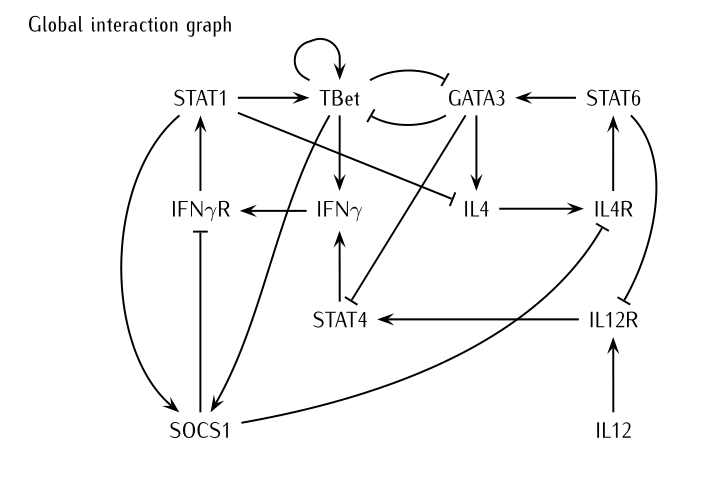
\includegraphics[height=0.9\textheight]{th_net}
\end{frame}
\begin{frame}[fragile=singleslide]{Bad results}
\footnotesize
		\begin{verbatim}
	IL4- : [['!SOCS1'], ['!TBet', '!GATA3']]
	TBet- : [['!GATA3']]
	STAT4+ : [['!GATA3'], ['IL12R']]
	STAT4- : [['!TBet', 'IFNg'], ['!TBet', '!GATA3']]
	GATA3+ : [['!TBet'], ['STAT6']]
	GATA3- : [['!TBet']]
	STAT1+ : [['IFNgR'], ['!TBet', '!GATA3']]
	STAT1- : [['!TBet', '!GATA3']]
	IFNgR+ : [['IFNg'], ['!SOCS1'], ['!TBet', '!GATA3']]
	IFNgR- : [['!TBet', '!GATA3']]
	SOCS1- : [['!TBet', '!GATA3']]
	IL4R+ : [['IL4'], ['!SOCS1'], ['!TBet', '!GATA3']]
	IL4R- : [['!TBet', '!GATA3']]
	IL12R+ : [['IL12'], ['!STAT6'], ['!TBet', '!GATA3']]
	STAT6+ : [['IL4R'], ['!TBet', '!GATA3']]
	STAT6- : [['!TBet']]
	\end{verbatim}
\end{frame}
\subsection{Hints}
\begin{frame}{Hints}
	Algorithm can be modified to take hints:
	\begin{itemize}
		\item Restrict possible influences to only some species
		\item Input from a priori knowledge
	\end{itemize}
\end{frame}
\begin{frame}{Hints (2)}
	With complete hints, results are perfect. (not shown because too big)
\end{frame}
\begin{frame}{Conclusion}
\begin{itemize}
	\item Existing framework from '84
	\item Promising for learning of boolean gene networks
	\item Can take into account previous knowledge of the system
\end{itemize}

\centering
\textit{Thank you ! Questions ?}
\end{frame}
\end{document}